\chapter{Introducción Específica} % Main chapter title

\label{Chapter2}

%----------------------------------------------------------------------------------------
%	SECTION 1
%----------------------------------------------------------------------------------------

\section{Definición del trabajo}

Al comienzo del Trabajo Final, y como parte de la asignatura \textit{Gestión de Proyectos}, se elaboró un plan de trabajo. Se incorporan en esta memoria aspectos relevantes de dicho trabajo.  En la sección \ref{sec:Objetivos} se definen los objetivos y alcances del proyecto.  En la sección \ref{sec:Requerimientos} se listan los requerimientos del sistema y los criterios de aceptación. Asimismo, se realizó un desglose de tareas a llevar a cabo en la que se estableció un cronograma para estas, según se puede apreciar en la sección \ref{sec:Gantt}. 

%-----------------------------------
%	SUBSECTION 1
%-----------------------------------
\subsection{Objetivos y alcances}
\label{sec:Objetivos}
%\vspace{10px}
\begin{itemize}

	\item \textbf{Objetivos}:\\
	Desarrollar un software que permita utilizar la plataforma CIAA como un controlador de acuarios. Agregar valor al ecosistema del proyecto CIAA incorporando nuevas aplicaciones para la plataforma.
	
	\item \textbf{Alcance}:\\
	El proyecto incluye únicamente el desarrollo de un software de control para la plataforma CIAA.

	\item \textbf{Restricciones}:\\
	Finalización del proyecto 1 de agosto de 2016.

	\item \textbf{Suposiciones}:\\
	Contar con los fondos solicitados al Ministerio de Industria Nacional permitirá costear los sensores y actuadores para armar una planta piloto de desarrollo.  En caso de que los fondos no estén disponibles tanto por el rechazo del proyecto presentado como por una demora en los plazos de adjudicación, está contemplado la utilización de simulaciones para emular los elementos que no se hayan podido adquirir.
	
	Asimismo, se estima que estará disponible durante el desarrollo del proyecto una plataforma CIAA-NXP.
	
	\end{itemize}
	
Cabe mencionar que las suposiciones respecto a los fondos no se cumplieron y se debieron ejecutar las acciones previstas para tal caso.

  

%-----------------------------------
%	SUBSECTION 3
%-----------------------------------
\clearpage
\subsection{Requerimientos y Criterios de aceptación}
\label{sec:Requerimientos}

Se listan a continuación los requerimientos del sistema de control de acuario. Estos serán retomados en la sección \ref{sec:Ensayos} para definir el plan de ensayos que permita verificar que los criterios de aceptación se cumplen satisfactoriamente.
 
\begin{itemize}
	\item \textbf{REQ1:}\\ El \textit{software} se debe desarrollar para la plataforma de \textit{hardware} CIAA, en Lenguaje C.
	\item \textbf{REQ2:}\\ El sistema debe poder medir las siguientes variables del entorno de un acuario:
	\begin{itemize}
		\item REQ2\_A: temperatura en el rango de 16 a 30 \grados C con una resolución de 0,5 \grados C o superior.
		\item REQ2\_B: pH en el rango mínimo de 5 a 9 con una resolución de 0,1 o superior.
%		\item REQ2\_C: nivel de agua alto o bajo.
	\end{itemize}
	\item \textbf{REQ3:}\\ El sistema debe poder actuar sobre los siguientes elementos del entorno de un acuario:
	\begin{itemize}
		\item REQ3\_A: Encender/apagar un artefacto de iluminación.
		\item REQ3\_B: Encender/apagar bombas para el llenado/vaciado de agua.
		\item REQ3\_C: Encender/apagar una bomba de $CO_2$.
%		\item REQ3\_C: Encender/apagar dosificador de alimento/nutrientes
		\item REQ3\_D: Encender/apagar un calefactor.
	\end{itemize}
	\item \textbf{REQ4:}\\ El equipo debe poder ser administrado mediante una interfaz web. Se debe poder visualizar el estado del sistema y realizar su programación.
	\item \textbf{REQ5:}\\ El equipo debe poder emitir una alarma por un medio adecuado, sonoro y/o visual, cuando las variables bajo control salgan de su rango de operación segura.
\end{itemize}

\textbf{Criterio de aceptación}:
	\begin{itemize}
		\item Correcta visualización de todas las variables de estado del sistema enumeradas en el REQ2 mediante una interfaz web.
		\item Correcto comportamiento al accionar los actuadores enumerados en el REQ3 desde la interfaz web.
	\end{itemize}

%-----------------------------------
%	SUBSECTION 4
%-----------------------------------
%
\subsection{Desglose de tareas / GANTT}
\label{sec:Gantt}

Como parte de la planificación se definieron las tareas necesarias para completar el trabajo y se establecieron las relaciones de correlatividad entre ellas.  Se presenta esta información en la forma de diagrama de Gantt.  En color azul oscuro se pueden ver las tareas del camino crítico.

\pagebreak[4]
\global\pdfpageattr\expandafter{\the\pdfpageattr/Rotate 90}

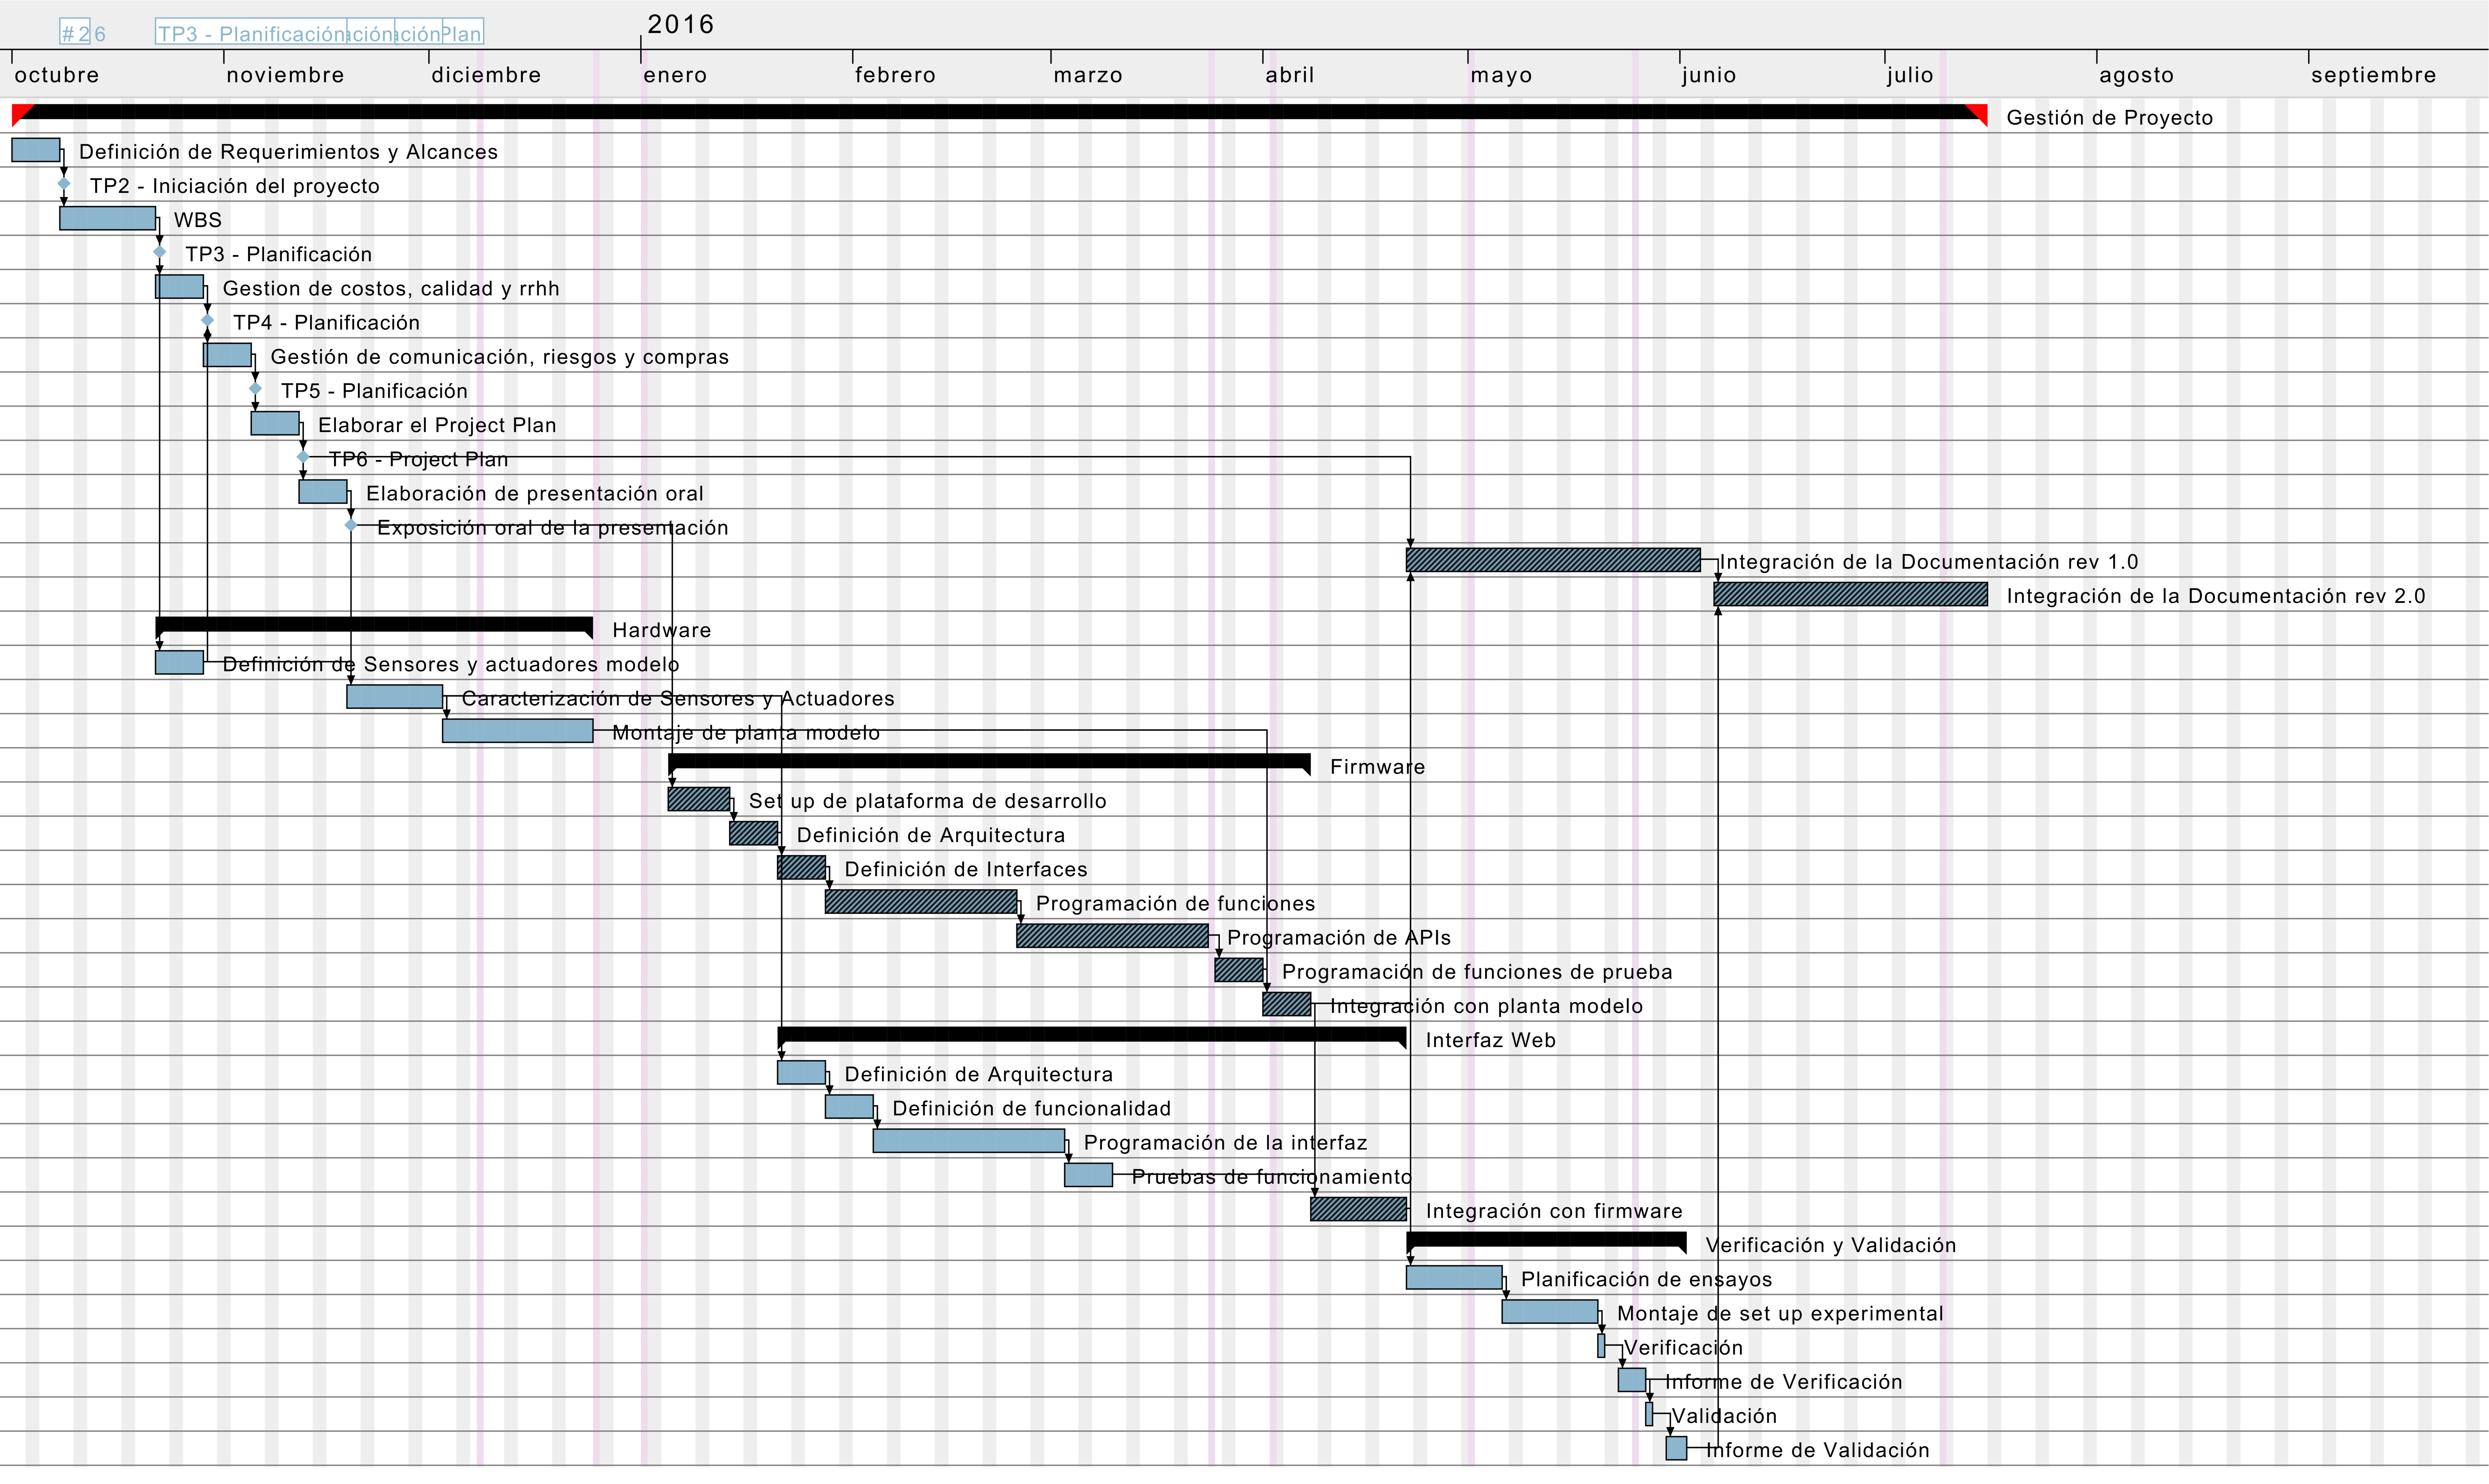
\includegraphics[width=1.1\paperwidth, angle = 90 ]{./Figures/gantt}


\clearpage
\pagebreak[4]\global\pdfpageattr\expandafter{\the\pdfpageattr/Rotate 0}
%----------------------------------------------------------------------------------------
%	SECTION 2
%----------------------------------------------------------------------------------------
\clearpage
\section{Planteo del problema}

Resulta necesario definir el modelo de control a utilizar y aclarar las suposiciones y limitaciones con que se trabajará. A su vez, se extienden los requerimientos definidos en la sección \ref{sec:Requerimientos} a la luz del análisis de la problemática que se pretende abordar.

Las variables que se deben medir son de naturaleza analógica y están asociadas a procesos físicos lentos.   En este sentido, se adopta en principio una tasa de muestreo de 1 Hz para la adquisición de dichas variables. 

Se definen valores umbrales límite para las variables medidas y se establecen condiciones de alarma.  Se definen dos alarmas por cada variable medida, una por exceso, en caso de que se supere el valor máximo permitido y otra por defecto, para el caso en que la variable se encuentre por debajo del valor umbral mínimo.

Dado que la planta que se utiliza para el desarrollo del \textit{firmware} no es un acuario real, en el presente trabajo no se profundiza sobre la dinámica del acuario en sí mismo.  En los lazos de control se aplican acciones binarias del tipo encender/apagar sobre los actuadores del sistema en función de las condiciones de alarma presentes. 

Las acciones de control se deben sostener en el tiempo mientras la condición de alarma que las haya iniciado esté presente. Asimismo, cuando haya alguna acción iniciada por el control de una condición de alarma, el estado del actuador siendo operado no debe poder ser cambiado manualmente, tanto para encenderse como apagarse, según sea el caso. Cuando no haya alarmas controlando un determinado actuador, este se debe poder operar manualmente.


\subsection{¿Qué hace falta medir, actuar, alertar?}

En esta sección se definen los sensores, actuadores y alarmas que serán parte del sistema de monitoreo y control.  En la tabla \ref{tab:sensores} se declaran los sensores con las características principales que deben tener. Se declaran las condiciones de alarma, asociadas a los valores máximos y mínimos de cada sensor, en la tabla \ref{tab:alarmas}. En la tabla \ref{tab:actuadores} se declaran los actuadores del sistema con las características principal que deben tener.   

\vspace{30px}

\begin{table}[ht]
	\centering
	\caption{Declaración de Sensores.}
	\begin{tabular}{@{} l *3c @{}}    \toprule
		\emph{\textbf{Nombre}} & \emph{\textbf{Rango}} & \emph{\textbf{Unidad}}  & \emph{\textbf{Resolución}}  \\
		\midrule
		Nivel de agua	& 0 - 20 	& cm		 	& 0,1 cm\\		
		Temperatura		& 16 - 30	& \grados C 	& 0,5 \grados C\\
		pH				& 5 - 9		& -			& 0,1 \\ 
		\bottomrule
		\hline
	\end{tabular}
	\label{tab:sensores}
\end{table}

\begin{table}[ht]
	\centering
	\caption{Declaración de Alarmas.}
	\begin{tabular}{@{} l l l@{}}    \toprule
		\emph{\textbf{Nombre}} & \emph{\textbf{Sensor asociado}} & \emph{\textbf{Condición}}  \\\midrule
		Nivel de agua alto	& Nivel de agua 	& $>$ 15 cm\\		
		Nivel de agua bajo	& Nivel de agua	& $<$ 5 cm\\
		Temperatura alta		& Temperatura	& $>$ 21,5 \grados C\\
		Temperatura baja		& Temperatura	& $<$ 17,5 \grados C\\
		Valor de pH alto		& pH				& $>$ 7,5\\ 
		Valor de pH bajo		& pH 			& $<$ 6,5\\	 \bottomrule
		\hline
	\end{tabular}
	\label{tab:alarmas}
\end{table}


\begin{table}[ht]
	\centering
	\caption{Declaración de Actuadores.}
	\begin{tabular}{@{} l *2c @{}}    \toprule
		\emph{\textbf{Nombre}} 	&  &   \\\midrule
		Bomba de entrada de agua	&  	& \\		
		Bomba de entrada de agua	&	& \\
		Calefactor				&	& \\
		Iluminación				& 	& \\
		Bomba de $O_2$			& 	& \\ 
		Bomba de $CO_2$			&  	& \\	 \bottomrule
		\hline
	\end{tabular}
	\label{tab:actuadores}
\end{table}



\subsection{Modelación de la dinámica de acuario}

Como ya fuera mencionado, la dinámica del acuario está fuera de los alcances del presente trabajo. Sin embargo, resulta necesario adoptar un modelo, si bien sencillo, mínimamente realista para describir la evolución de las variables de estado del sistema cuando los actuadores se encuentran en funcionamiento. Por este motivo, se describen los efectos esperables de los actuadores sobre el sistema.

Las bombas de entrada y salida de agua hacen variar el nivel de agua a la misma tasa pero en distinto sentido.  Se asume que si ambas se encuentran en funcionamiento el nivel de agua no se modifica significativamente.  Para aumentar o disminuir el nivel de agua del acuario se debe encender la bomba de entrada y apagar la de salida o viceversa, respectivamente.

El funcionamiento del calefactor incrementa la temperatura del agua del acuario.  Para disminuir la temperatura se debe recircular el agua encendiendo simultáneamente ambas bombas de agua.  Se asume que en esta situación el agua que ingresa al acuario tiene menor temperatura que la que egresa.

La iluminación y la bomba de $O_2$ no tienen efectos mensurables sobre las variables que miden nivel, temperatura ni valor de pH del agua.

El funcionamiento de la bomba de $CO_2$ disminuye el pH del agua del acuario, es decir, la vuelve más ácida.  Para restituir el valor de pH del agua a la neutralidad, en caso de que esta se encuentre demasiado ácida, se debe recircular el agua encendiendo simultáneamente ambas bombas de agua.  Se asume que el agua que ingresa al acuario tiene pH neutro.




\subsection{Alternativas tecnológicas}

En esta sección se presentan las alternativas tecnológicas que se evaluaron para los sensores en base a los requerimientos y la disponibilidad en el mercado local. Se consultaron tiendas de acuarios para conocer el estado del arte y los sensores que pudieran conectarse a un sistema de control electrónico. El relevamiento no pretende ser exhaustivo sino proporcionar una guía confiable para el desarrollo del \textit{firmware} de control.

Existen múltiples maneras de medir el nivel de agua en un recipiente.  En cuanto a los principios de funcionamiento de los sensores más utilizados se pueden mencionar:

\begin{itemize}
\item Detección mecánica de nivel mediante el cierre de un contacto por la acción de un flotador o boya.  Proporciona un valor binario que indica si el nivel de agua llegó hasta el punto que acciona el contacto o no.  Un sensor de este tipo se puede observar en la figura \ref{fig:Sensor de nivel1}.
\item Utilización de la presión hidroestática del fluido para determinar la altura de la columna de agua.  En la figura \ref{fig:Sensor de nivel2} se muestra un ejemplo de este tipo de sensor cuya salida es un valor de resistencia proporcional al nivel de agua.
%\item Radar o Ultrasónido para medir distancia a la interfaz agua-aire.
\end{itemize}

\begin{figure}[h]
\centering
\begin{subfigure}{.5\textwidth}
  \centering
    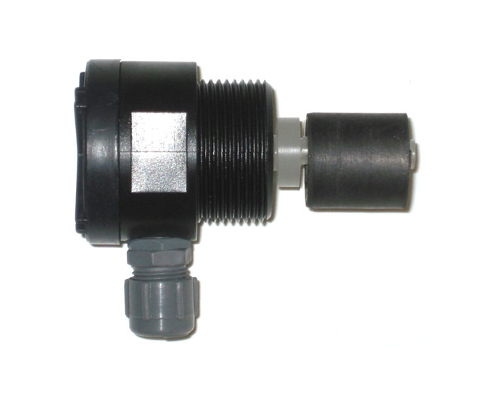
\includegraphics[height=.15\textheight]{./Figures/sensor_nivel_1}
\caption[]{Electrol serie 5025 \protect\footnotemark}	
	\label{fig:Sensor de nivel1}
	
\end{subfigure}%
\begin{subfigure}{.5\textwidth}
  \centering
  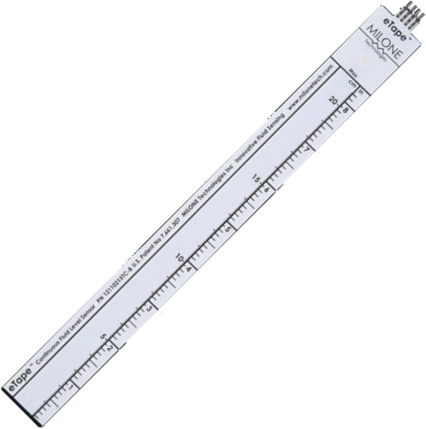
\includegraphics[height=.15\textheight]{./Figures/sensor_nivel_3}
  	\caption[]{Milonetech eTape \protect\footnotemark}
  \label{fig:Sensor de nivel2}
\end{subfigure}
\caption[Alternativas comerciales de sensores de nivel.]{Alternativas comerciales de sensores de nivel.}
\label{fig:sensoresnivel}
\end{figure}

\footnotetext[1]{\url{http://www.electrolsrl.com.ar/docs/5025-01D.pdf}}

\footnotetext{\url{http://milonetech.com/p/about-etape}}

Para la medición de la temperatura del agua del acuario se encontraron principalmente sensores de temperatura tipo termistor NTC (\textit{Negative Temperature Coefficient}). El principio de funcionamiento se basa en presentar un valor de resistividad que disminuye con el incremento de la temperatura.  En la figura \ref{fig:temperatura1} se puede observar un sensor de este tipo de 10 $k\Omega$ a 25 \grados C en un encapsulado de acero inoxidable sumergible con un cable de 30 cm.  

Por otra parte, se encontró un termómetro digital basado en el integrado DS18B20 que proporciona lecturas de la temperatura de 9 a 12 bits en forma configurable, sobre una interfaz ``1-Wire'' \citep{dallas:ds18b20} que requiere un solo un cable de señal conectado al microcontrolador. En la figura \ref{fig:temperatura2} se puede observar un sensor de este tipo que también cuenta con un encapsulado de acero inoxidable apto para inmersión con un cable de 90 cm.

\vspace{10px}

\begin{figure}[h]
\centering
\begin{subfigure}{.5\textwidth}
  	\centering
  	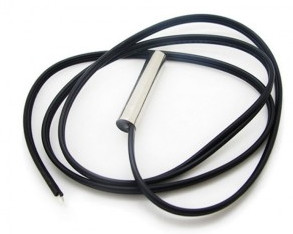
\includegraphics[height=.15\textheight]{./Figures/sensor_temp_1}
	\caption{Termistor NTC\protect\footnotemark}
	\label{fig:temperatura1}
\end{subfigure}%
\begin{subfigure}{.5\textwidth}
	\centering
  	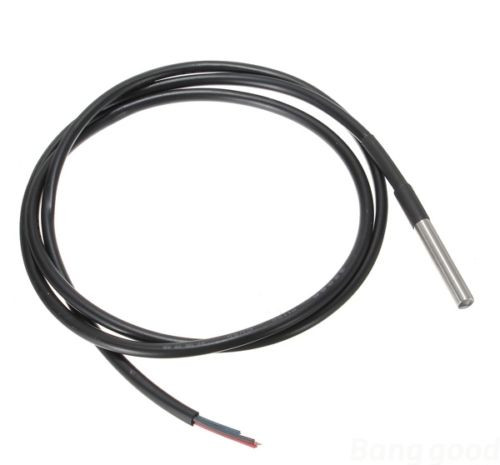
\includegraphics[height=.15\textheight]{./Figures/sensor_temp_2}
  	\caption[]{Termómetro digital DS18B20\protect\footnotemark}
  	\label{fig:temperatura2}
\end{subfigure}
\caption[Alternativas comerciales de sensores de temperatura.]{Alternativas de sensores de temperatura. }
\label{fig:sensoresTemp}
\end{figure}



Se halló una sonda compuesta por un electrodo de vidrio combinado con una membrana de Ag/AgCl (plata / cloruro de plata),  que se puede utilizar en una variedad de mediciones de pH. En la figura \ref{fig:sensor_pH1} se puede apreciar la sonda para las mediciones de pH. En la figura \ref{fig:sensor_pH2} se muestra un detalle del electrodo. Este instrumento provee una señal analógica lineal en el rango de pH 0-14 y es apto para mediciones \textit{online} por tiempo prolongado (1 año) \citep{sensor_pH}. Debe ser calibrado periódicamente con una solución de referencia.

\footnotetext[3]{\url{https://www.openhacks.com/uploadsproductos/im120628010_2.jpg}}

\footnotetext{\url{https://www.openhacks.com/uploadsproductos/_igp1391-500x500.jpg}}

\vspace{10px}

\begin{figure}[h]
\centering
\begin{subfigure}{.5\textwidth}
  	\centering
    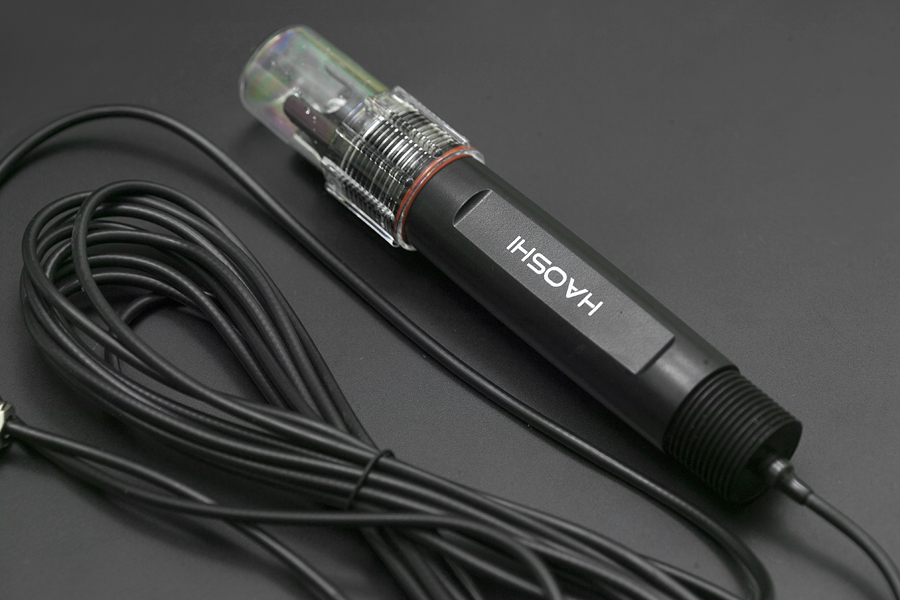
\includegraphics[height=.2\textheight]{./Figures/sensor_pH1}
	\caption[]{Sonda para la medición de pH\protect\footnotemark .}
	\label{fig:sensor_pH1}
\end{subfigure}%
\begin{subfigure}{.5\textwidth}
	\centering
    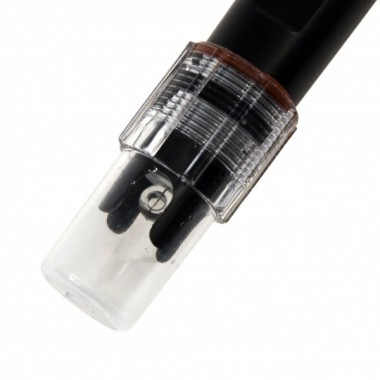
\includegraphics[height=.2\textheight]{./Figures/sensor_pH2}
	\caption[]{Detalle del electrodo para medir pH\protect\footnotemark .}
	\label{fig:sensor_pH2}
\end{subfigure}
\caption{Sonda comercial para la medición de pH.}
\label{fig:sensores_pH}
\end{figure}


\footnotetext[5]{\url{http://www.dfrobot.com/wiki/images/f/f4/DFR0169_picture.JPG}}
\footnotetext{\url{https://www.openhacks.com/uploadsproductos/_dsc0555-600x600.jpg}}




